\section{Badania}
W~niniejszym rozdziale opisany został przebieg przeprowadzonych badań oraz analiza ich wyników. W~kolejnych podrozdziałach zostaną przedstawione kolejne różne eksperymenty. Dokładne otrzymane wyniki znajdują się na~dołączonej do pracy płycie~CD w~odpowiednich plikach, o~nazwach zgodnych z~podrozdziałem opisującym dane badanie i~jego wyniki.

%\subsection{Opóźnienia pojedynczego odcinka sieci}
%\subsection{Wpływ topologi na opóźnienia}
\subsection{Czas stabilizacji sieci po odłączeniu i~podłączeniu dowolnego urządzenia}
Badanie miało na~celu sprawdzenie czy zgodnie z~zapewnieniami producenta możliwe jest rozłączanie i~ponowne podłączanie urządzeń do~sieci ,,w locie'' bez konieczności żadnej dodatkowej ingerencji. Do przeprowadzenia pomiarów autor odłączał przewód ethernetowy i~podłączał go~ponownie do~gniazda. Oczywiście taka metoda może mieć wpływ na~dokładność dokonywanych pomiarów, ale zdaniem autora jest on stosunkowo niewielki, ze względu na fakt, że od~momentu odłączenia do wykrycia tego zajścia przez urządzenie nadzorujące pracę sieci mija pewien czas, który w optymistycznym przypadku może być krótszy niż sam proces ingerencji autora. Aby poprawić dokładność należałoby zastosować specjalnie stworzone samodzielnie urządzenie, co zostanie opisane w~perspektywach rozwoju niniejszej pracy. Wszystkie zmierzone czasy oraz treści komunikatów zostały odczytane w~środowisku TwinCAT System Manager, przykładowy został przedstawiony na Rysunku~\ref{reading_time}.

\begin{figure}[!htb] 	\centering 	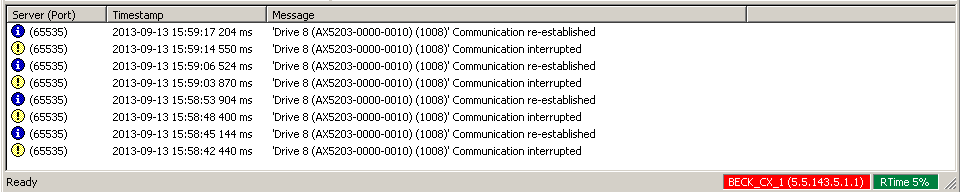
\includegraphics[width=0.95\textwidth]{images/reading_time} \caption{Topologia stanowiska z odłączonym jednym węzłem} \label{reading_time} \end{figure}
\vspace{-5mm}
\subsubsection{Pojedyncze urządzenie}
Eksperyment miał na~celu sprawdzenie po upływie jakiego czasu oo~odłączenia i~ponownego podłączenia pojedynczego węzła sieci zaczyna on~znów funkcjonować poprawnie. Zaburzoną pracę sieci przedstawiono na~Rysunku~\ref{one_slave}, który został wygenerowany przy użyciu środowiska TwinCAT System Manager, które udostępnia możliwość podglądu topologii sieci w~czasie rzeczywistym. Do eksperymentu wybrany został węzeł końcowy w~topologii.
\begin{figure}[!htb] 	\centering 	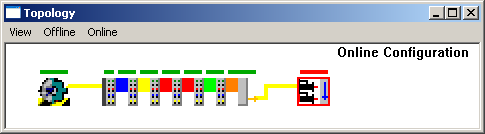
\includegraphics[width=0.9\textwidth]{images/topologyCXerror} \caption{Topologia stanowiska z odłączonym jednym węzłem} \label{one_slave} \end{figure}

\begin{table}[!htb]
\begin{center}
\begin{tabular}{| c | c | c | c | c |}\hline
\textbf{Liczba} & \textbf{Wartość} & \textbf{Wartość} & \textbf{Wartość} & \textbf{Odchylenie} \\
\textbf{próbek} & \textbf{średnia} & \textbf{minimalna} & \textbf{maksymalna} & \textbf{standardowe} \\\hline\hline
20 & 2,715s & 2,644s & 3,184s & 0,131\\\hline
\end{tabular}
\end{center}
\vspace*{-6mm}
  \caption{Wyniki przeprowadzonego badania}
	\label{badania:wyniki:stabilizacja_jeden}
\end{table}

\noindent Wyniki przeprowadzonego eksperymentu zostały zebrane w Tabeli~\ref{badania:wyniki:stabilizacja_jeden}. Na podstawie zmierzonych wartości oraz po ich analizie statystycznej uzyskano wykres przedstawiony na Rysunku~\ref{badania:wykres:stabilizacja_jeden}
\begin{figure}[htbp]
 \centering
 \begin{tikzpicture}[x=0.5cm,y=2cm]
  \tikzstyle{background grid}=[draw, black!50,step=.25cm]
	\draw[-latex, thin, draw=gray] (0,0)--(20,0) node [right] {$x$};
	\draw[-latex, thin, draw=gray] (0,0)--(0,4) node [above] {$t[s]$};
	%\draw [dotted, gray, step=0.5cm] (0,0) grid (20,4);
 
	\draw[thick] (0,2.678)--(20,2.678) node[left=10cm] {2,678};
	\draw[thin, dotted] (0,2.664)--(20,2.664) node[below] {min};
	\draw[thin, dotted] (0,2.774)--(20,2.774) node[above] {max};
		
	\node at (1, 2.664) {\textbullet};
	\node at (2, 2.664) {\textbullet};
	\node at (3, 2.654) {\textbullet};
	\node at (4, 2.664) {\textbullet};
	\node at (5, 2.654) {\textbullet};
	\node at (6, 2.774) {\textbullet};
	\node at (7, 2.764) {\textbullet};
	\node at (8, 2.664) {\textbullet};		
	\node at (9, 2.654) {\textbullet};
	\node at (10, 2.664) {\textbullet};
	\node at (11, 2.654) {\textbullet};
	\node at (12, 2.664) {\textbullet};
%	\node at (13, 2.774) {\textbullet};
%	\node at (14, 2.774) {\textbullet};
%	\node at (15, 2.774) {\textbullet};
%	\node at (16, 2.774) {\textbullet};							
%	\node at (17, 2.774) {\textbullet};
%	\node at (18, 2.774) {\textbullet};
%	\node at (19, 2.774) {\textbullet};
%	\node at (20, 2.774) {\textbullet};
					
\end{tikzpicture}
\caption{Pomiary czasu ponownego podłączenia oraz obliczona wartość średnia}
\label{badania:wykres:stabilizacja_jeden}
\end{figure}

Analiza wyników przeprowadzonego badania potwierdza, że istnieje możliwość odłączenie i~ponowne podłączenie pojedynczego węzła sieci ,,w locie''. Czas potrzebny na~stabilizację połączenia po jego utracie jest zdaniem autora zadowalający. Obserwując uzyskany wykres można dojść do wniosku, że różnice pomiędzy kolejnymi iteracjami eksperymentu są stosunkowo małe, o czym świadczy odchylenie standardowe, którego wartość wynosi 0,131. Zdaniem autora głównym źródłem różnic jest zastosowana metoda pomiarowa.

\subsubsection{Wyspa z modułami I/O}
Eksperyment miał na~celu sprawdzenie po upływie jakiego czasu od~odłączeniu i~ponownego podłączenia zdalna wyspa z~dołączonymi kilkoma modułami wejścia/wyjścia zaczyna w~całości działać poprawnie tzn. wszystkie węzły nawiązują komunikację. Zaburzoną pracę sieci przedstawiono na~Rysunku~\ref{coupler}.
\begin{figure}[!htb] 	\centering 	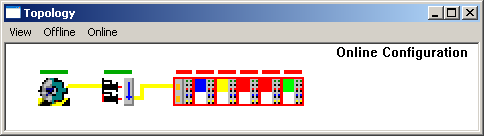
\includegraphics[width=0.8\textwidth]{images/topologyCPerror} \caption{Topologia stanowiska z odłączoną wyspą} \label{coupler} \end{figure}
%1,5s wyspa i każdy kolejny moduł I/O z opóźnieniem 4ms

Wyniki przeprowadzonego eksperymentu zostały zebrane w Tabeli~\ref{badania:wyniki:stabilizacja_wyspa}.
\begin{table}[!htb]
\begin{center}
\begin{tabular}{| c | c | c | c | c |}\hline
\textbf{Liczba} & \textbf{Wartość} & \textbf{Wartość} & \textbf{Wartość} & \textbf{Odchylenie} \\
\textbf{próbek} & \textbf{średnia} & \textbf{minimalna} & \textbf{maksymalna} & \textbf{standardowe} \\\hline\hline
42 & 2,699s & 2,634s & 2,812s & 0,061s \\\hline
\end{tabular}
\end{center}
\vspace*{-6mm}
  \caption{Wyniki przeprowadzonego badania}
	\label{badania:wyniki:stabilizacja_wyspa}
\end{table}

Na podstawie zmierzonych wartości oraz po ich analizie statystycznej uzyskano wykres przedstawiony na Rysunku~\ref{badania:wykres:stabilizacja_wyspa}. Kolejnymi kolorami są oznaczone kolejne iteracje badania, a~punkty tego samego koloru oznaczają kolejne węzły zdalnej stacji wejść/wyjść.
\begin{figure}[htbp]
 \centering
 \begin{tikzpicture}[x=0.5cm,y=10cm]


 \draw[latex-latex, thin, draw=gray] (0,1.25)--(20,1.25) node [right] {$x$}; % l'axe des abscisses
 \draw[latex-latex, thin, draw=gray] (0,1.25)--(0,2) node [above] {$y$}; % l'axe des ordonnées
 \draw[thick] (0,1.5)--(20,1.58); % l'axe des abscisses

    \foreach \i in {0,...,20}{% 
\foreach \Point in {(\i ,1.5+0.004*\i)}{
    \node at \Point {\textbullet}; } ;}     

% to ensure that the points are being properly centered:
\draw [dotted, gray] (0,1.25) grid (20,2);

\end{tikzpicture}
\caption{Współczynnik wykorzystania kanału transmisyjnego w Ethernecie (dwa pierwsze wykresy od lewej strony) i EtherCAT}
\label{etherCAT:wykorzystanie}
\end{figure}

Spoglądając na uzyskane wyniki oraz wykres można zaobserwować, że zwiększenie liczby odłączanych i~podłączanych ponownie węzłów nie~wpłynęło na~możliwość dokonywania tej operacji w~czasie pracy sieci. Ciekawa zdaniem autora jest różnica czasu pomiędzy podłączeniem się pierwszego urządzenia z~zestawu, a~każdym kolejnym wynoszący 2 lub milisekundy. Tak więc liczba modułów wejścia/wyjścia ma~proporcjonalnie niewielki wpływ na czas potrzebny do ustabilizowania się całego zdalnego zestawu.

\subsubsection{Wszystkie węzły sieci}
\label{badania:cala_siec}
Eksperyment miał na~celu sprawdzenie po upływie jakiego czasu od~odłączeniu i~ponownego podłączenia wszystkich węzłów sieć wróci ona do~normalnego stanu. Zaburzoną pracę sieci przedstawiono na~Rysunku~\ref{topologyCPallerror}.
\begin{figure}[!htb] 	\centering 	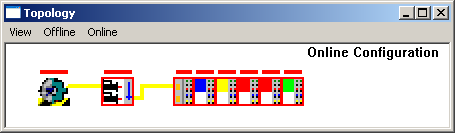
\includegraphics[width=0.9\textwidth]{images/topologyCPallerror} \caption{Topologia stanowiska z odłączonymi wszystkimi węzłami} \label{topologyCPallerror} \end{figure}

\noindent Stan sieci bezpośrednio po ponownym podłączeniu kabla sieciowego i~w~fazie inicjalizacji ponownego połączenia przedstawiono na Rysunku~\ref{topologyCPallloading}. Można zaobserwować, że węzły połączone w~zdalną stację wejść/wyjść są już w~jednej z~kolejnych faz inicjalizacji, a~pozostałe jeszcze nie rozpoczęły.
\begin{figure}[!htb] 	\centering 	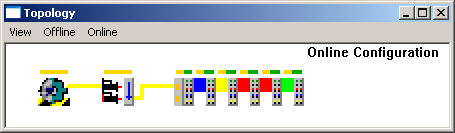
\includegraphics[width=0.9\textwidth]{images/topologyCPallloading} \caption{Topologia stanowiska w czasie ponownego podłączania węzłów} \label{topologyCPallloading} \end{figure}

\begin{table}[!htb]
\begin{center}
\begin{tabular}{| c | c | c | c | c |}\hline
\textbf{Liczba} & \textbf{Wartość} & \textbf{Wartość} & \textbf{Wartość} & \textbf{Odchylenie} \\
\textbf{próbek} & \textbf{średnia} & \textbf{minimalna} & \textbf{maksymalna} & \textbf{standardowe} \\\hline\hline
10 & 4,790s & 4,149s & 5,455s & 0,446s\\\hline
\end{tabular}
\end{center}
\vspace*{-6mm}
  \caption{Wyniki przeprowadzonego badania}
	\label{badania:wyniki:stabilizacja_siec}
\end{table}

\noindent Wyniki przeprowadzonego eksperymentu zostały zebrane w Tabeli~\ref{badania:wyniki:stabilizacja_jeden}. Na podstawie zmierzonych wartości oraz po ich analizie statystycznej uzyskano wykres przedstawiony na Rysunku~\ref{badania:wykres:stabilizacja_siec}
\begin{figure}[h]
 \centering
 \begin{tikzpicture}[x=1cm,y=5cm]
  \tikzstyle{background grid}=[draw, black!50,step=.25cm]
	\draw[-latex, thin, draw=gray] (0,4)--(10,4) node [right] {$x$};
	\draw[-latex, thin, draw=gray] (0,3.95)--(0,5.55) node [left] {$t[s]$};
	%\draw [dotted, gray, step=0.5cm] (0,0) grid (20,4);
 	\draw (0,4) node[left] {4};
	\draw[] (0,4.790)--(10,4.790) node[left=10cm] {4,790};
	\draw[thin, dotted] (0,4.149)--(10,4.149) node[below] {min};
	\draw[thin, dotted] (0,5.455)--(10,5.455) node[above] {max};
		
	\node at (1, 4.863) {\textbullet};
	\node at (2, 4.149) {\textbullet};
	\node at (3, 5.313) {\textbullet};
	\node at (4, 5.455) {\textbullet};
	\node at (5, 4.339) {\textbullet};
	\node at (6, 4.911) {\textbullet};
	\node at (7, 5.099) {\textbullet};
	\node at (8, 4.339) {\textbullet};		
	\node at (9, 4.967) {\textbullet};
	\node at (10, 4.463) {\textbullet};
					
\end{tikzpicture}
\caption{Pomiary czasu ponownego podłączenia oraz obliczona wartość średnia.}
\label{badania:wykres:stabilizacja_siec}
\end{figure}

Analiza wyników przeprowadzonego badania pozwala wysnuć wniosek, że możliwe jest całkowite rozłączenie i~ponowne podłączenie sieci ,,w locie''. Czas potrzebny na~stabilizację połączenia po jego utracie również w tym wypadku jest zdaniem autora zadowalający. Niestety jednak porównując uzyskane wielkości do~tych z~badania pojedynczego węzła sieci można zauważyć, że czas ten wzrósł dość znacząco i~w~przypadku jeszcze większej liczby węzłów przestanie on już być akceptowalny. Obserwując uzyskany wykres można dojść do wniosku, że różnice pomiędzy kolejnymi iteracjami eksperymentu są stosunkowo małe i~wpływ na~nie może mieć w~większości zastosowana metoda pomiarowa.

\clearpage
\subsubsection{Problemy}
W~czasie dziesiątek przeprowadzonych w~tym badaniu pomiarów autor doprowadził do sytuacji w~której sieć nie~powróciła już samoczynnie do~prawidłowego działania. Jest to sprzeczne z~zapewnieniami twórców standardu i~dlatego wszystkie przypadki zostaną tu zawarte,szczegółowo opisane i~przeanalizowane.

\begin{enumerate}
\item Treść wiadomości odczytanej ze środowiska była następująca: \textit{Device 2 (EtherCAT (v2.10 only)': 'INIT to PREOP' failed! Error: 'read slave count'. Communication Error '0x707 (1799)'.} \\[1mm]
%ADS, problem ze stanem urządzenia
Do błędu doszło w~momencie zaburzenia pracy całej sieci, tj. odłączenia wszystkich węzłów podrzędnych od węzła nadrzędnego jak w~badaniu~\ref{badania:cala_siec}. Stan sieci po~wystąpieniu błędu przedstawiono na Rysunku~\ref{err0x707}.
\begin{figure}[!htb] 	\centering 	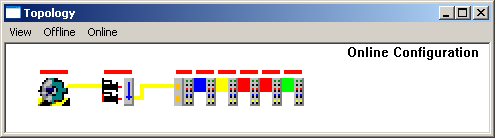
\includegraphics[width=0.9\textwidth]{images/err0x707} \caption{Stan sieci po błędzie 0x707} \label{err0x707} \end{figure}

Na rysunku można zaobserwować, że urządzenia są podłączone do sieci, ale ich stan jest błędny (brak czerwony ramek wokół węzłów). Analizując stan stanowiska i~sieci w~środowisku zaobserwowano, że w~sieci nie są przesyłane dane.
Dalsza analiza wykazała, że węzeł AX-5203 jest w prawidłowym stanie inicjalizacji (0x0001), natomiast problematyczna okazała się zdalna wyspa, która ma nieprawidłowy stan 0x5C01, który według jednej z dokumentacji producenta oznacz błąd podczas resetowania stanu \cite{err0x707}.
Okazało się, ze problem ten można prosto rozwiązać bez potrzeby restartowania całego stanowiska poprzez wymuszenie zmiany stanu węzła nadrzędnego z~INIT na~OP (opcja dostępna z~poziomu środowiska), co skutkuje wysłaniem takiego samego żądania do wszystkich węzłów podrzędnych i sieć ponownie zaczyna funkcjonować. Wynik analizy znajduje odzwierciedlenie bezpośrednio w~treści wiadomości opisującej błąd.
\end{enumerate}

\subsection{Badania niewykonalne}

\subsubsection{Zbadanie innych topologii}

\subsubsection{Zbadanie opóźnień na poziomie transmisji pojedynczych ramek}
%Różne kable
%Długość kabla
%
%Połączyć do jednego sterownika oba napędy kolejno i zrobić coś na zasadzie inkrementacji i sprawdzić czy się przypadkiem nie rozjedzie
%
%Mamy opóźnienie na jednym odcinku
%
%Ewentualnie jeden kabel można zamienić na dłuższy i sprawdzić czy nie ma różnicy.
%
%Wymyślić jak sprawdzić czas ponownego włączenia do sieci.